\section{\esp Introdução}

No início do século XVIII, especula-se que, na cidade russa de Königsberg, eram constituídas quatro áreas, as quais eram separadas pelo Rio Pregel. No entanto, o deslocamento dos cidadãos era complexo devido a utilização de barcos para tal. Assim sendo, foram construídas sete pontes conforme ilustrado na figura 1, para auxiliar na locomoção destes entre as ilhas e suas margens. Contudo, o trajeto ainda se tornava árduo e tais pessoas da época começaram a se questionar se era possível cruzar as pontes apenas uma vez e, se possível, retornar ao ponto inicial.

\begin{figure}[ht]
	\centering	
	\caption[\hspace{0.1cm}Esboço da cidade de Königsberg.]{Esboço da cidade de Königsberg}
	\vspace{-0.4cm}
	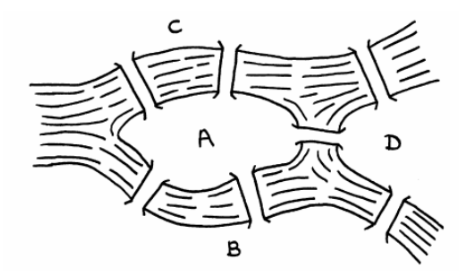
\includegraphics[width=0.6\textwidth]{figuras/cidade.png}
	 \vspace{-0.2cm}
	\\\textbf{\footnotesize Fonte: Hopkins; Wilson, 2004, p. 198}
	\label{fig:figura1}
\end{figure}

O grande matemático suiço Leonhard Euler, chega à Rússia no ano de 1730 para exercer o cargo de Filosofia Natural na Academia de Ciências de São Petersburgo. No entanto, após três anos tornou-se o principal matemático da academia com a saída de Daniel Bernoulli.

Com sua ascensão, o prefeito próximo a cidade de Königsberg enviou-lhe uma carta datada de 09 de março de 1736 em nome de Heinrich Kiihn, um matemático local que explica a questão das pontes. Intrigado com a questão Euler envia uma carta a Giovanni Jacopo Marinoni, um matemático e engenheiro italiano repassando a questão e dizendo em sua carta:

\begin{citacaodireta}
Um problema me foi apresentado sobre uma ilha na cidade de Konigsberg, cercada por um rio, atravessado por sete pontes, e foi me perguntado se alguém poderia atravessar as pontes separadas em uma caminhada contínua de tal forma que cada ponte fosse atravessada apenas uma vez. Fui informado que até então ninguém havia demonstrado a possibilidade de fazer isso, ou mostrado que é impossível. Esta questão é tão banal, mas pareceu-me digno de atenção em que nem a geometria, álgebra, ou mesmo a arte de contar foram suficientes para resolvê-lo (HOPKINS; WILSON, 2004, p. 201).
\end{citacaodireta}

Euler então monta um modelo matemático representando o mapa da cidade, associando cada ilha a um ponto e cada ponte como uma linha que interliga esses pontos.  Desta forma originalizando a Teoria dos Grafos com base na figura 2 ilustrada abaixo:

\begin{figure}[ht]
	\centering	
	\caption[\hspace{0.1cm}Grafo que representa a cidade de Königsberg.]{Grafo que representa a cidade de Königsberg}
	\vspace{-0.4cm}
	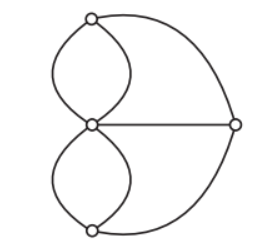
\includegraphics[width=0.3\textwidth]{figuras/grafo-cidade.png}
	 \vspace{-0.2cm}
	\\\textbf{\footnotesize Fonte: Desenvolvido pelo autor}
	\label{fig:figura1}
\end{figure}

Esta figura representa seus pontos como vértices e suas ligações como arestas, denominando um grafo. Euler percebe durante seu raciocínio que existem vértices com exatamente três arestas incidentes. Entretanto, os cidadãos gostariam de atravessar cada ponte apenas uma única vez, mas cada vértice deveria conter um número par de arestas, tornando impossível o percurso seguindo as restrições da população.

Com a resolução desta questão que indica que se e somente, se o grafo possuir números pares de arestas é possível passar uma única vez pelo caminho. Euler, então envia sua resposta ao prefeito em 03 de abril de 1736 da seguinte forma:

\begin{citacaodireta}
Assim você vê, mais nobre senhor, como este tipo de solução tem pouca relação com a matemática, e eu não entendo por que você espera que um matemático possa produzi-la, ao invés de qualquer outra pessoa, já que a solução baseia-se na razão e sua descoberta não depende de qualquer princípio matemático. Devido a isso, eu não sei por que questões comuns que têm tão pouca relação com a matemática são resolvidas mais rapidamente pelos matemáticos do que por outros (HOPKINS; WILSON, 2004, p. 201).
\end{citacaodireta}

Apesar de não vincular sua resolução do problema à matemática, Euler se interessou em divulgar sua análise para a comunidade científica da época. Na qual foi homenageado com parte de seu nome no Teorema dos Caminhos Eulerianos. Passado algum tempo começaram a surgir novos problemas, como o do Caixeiro Viajante, o das Quatro Cores e o do Carteiro Chinês, que permitiram o desenvolvimento da Teoria dos Grafos.

\section{\esp CONCEITOS SOBRE GRAFOS}

Como toda teoria matemática, a Teoria dos Grafos contém diversas nomenclaturas e termos técnicos. Nesta seção são apresentadas algumas de suas definições principais para o entendimento completo deste estudo.

\subsection{\esp Estruturas de um Grafo}

Grafo é uma representação abstrata de um conjunto de objetos e das relações existentes entre eles. Podendo ser descrito como um par de G (V,A) onde V é um conjunto não vazio de objetos denominados vértices e A é um conjunto de pares não ordenados de V, chamado arestas. Por exemplo, no grafo apresentado na figura 3 é apresentado um mapa de estradas e cidades.

\begin{figure}[ht]
	\centering	
	\caption[\hspace{0.1cm}Exemplo de um grafo.]{Exemplo de um grafo}
	\vspace{-0.4cm}
	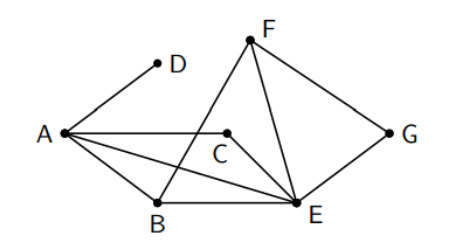
\includegraphics[width=0.3\textwidth]{figuras/exemplo-grafo.png}
	 \vspace{-0.2cm}
	\\\textbf{\footnotesize Fonte: Desenvolvido pelo autor}
	\label{fig:figura1}
\end{figure}

Pode-se destacar que dependendo da aplicação, as arestas do grafo podem ou não ser orientadas, ligar um vértice a ele próprio e ainda ter um peso (numérico) associado.

Grafos não orientados, ou simplesmente grafos, são compostos por dois vértices que são adjacentes se existir uma aresta conectando-os, ao passo que uma aresta é incidente aos vértices que ela conecta. 

\begin{figure}[ht]
	\centering	
	\caption[\hspace{0.1cm}Grafo não direcionado.]{Grafo não direcionado}
	\vspace{-0.4cm}
	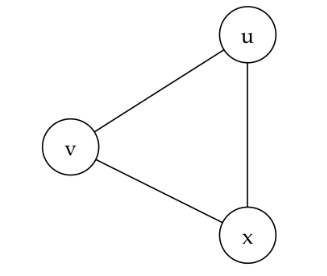
\includegraphics[width=0.3\textwidth]{figuras/grafo-nao-direcionado.png}
	 \vspace{-0.2cm}
	\\\textbf{\footnotesize Fonte: Desenvolvido pelo autor}
	\label{fig:figura1}
\end{figure}

Grafos orientados ou também conhecidos como dígrafos, dizemos que um vértice X é adjacente a um Y se, e somente se, (X,Y) pertence ao conjunto de arestas do grafo. No caso de incidência em grafos orientados, há de se considerar que a aresta (X,Y) é incidente somente em Y, enquanto a aresta (Y,X) incide em X.

\begin{figure}[ht]
	\centering	
	\caption[\hspace{0.1cm}Grafo direcionado ou dígrafo.]{Grafo direcionado ou dígrafo}
	\vspace{-0.4cm}
	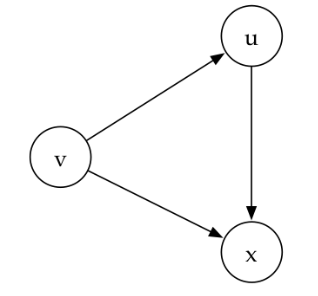
\includegraphics[width=0.3\textwidth]{figuras/grafo-direcionado.png}
	 \vspace{-0.2cm}
	\\\textbf{\footnotesize Fonte: Desenvolvido pelo autor}
	\label{fig:figura1}
\end{figure}

Grafos ponderados, possuem atribuição de pesos em suas arestas. São utilizados para determinar qual o melhor trajeto a adotar dado o problema. Supondo que para ir de um lugar para outro existem diversas estradas em que cada uma possui um pedágio e deseja-se escolher a estrada com menor valor de pedágio para chegar até o destino. O grafo da figura 6 exemplifica essa suposição.

\begin{figure}[ht]
	\centering	
	\caption[\hspace{0.1cm}Grafo ponderado.]{Grafo ponderado}
	\vspace{-0.4cm}
	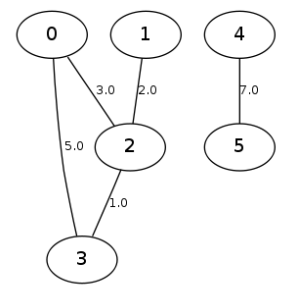
\includegraphics[width=0.3\textwidth]{figuras/grafo-ponderado.png}
	 \vspace{-0.2cm}
	\\\textbf{\footnotesize Fonte: Desenvolvido pelo autor}
	\label{fig:figura1}
\end{figure}

\subsection{\esp Representações}

Existem diversas maneiras de se representar grafos, cada uma com suas vantagens e desvantagens. Em algumas situações ou algoritmos nos quais pode-se utilizar de um grafo como entrada é necessário escolher uma representação específica. Neste estudo será utilizada a Lista de Adjacência e Matriz de Adjacência.
Para tal escolha pode-se utilizar de três critérios, sendo eles:

\begin{enumerate} 
 \item [a)] Quantidade de memória ou espaço gasto;
 \item [b)] Tempo gasto para determinar se um determinada aresta faz parte do grafo;
 \item [c)] Tempo gasto para encontrar os vizinhos de um vértice.
\end{enumerate}

A identificação dos vértices comumente não é feita pelo nome (como "Leonardo", "Belo Horizonte" ou "calça"), mas sim por um número. Ou seja, os vértices são numerados |V| de 0 até |V| -1. Um exemplo de grafo é uma rede social, no qual as pessoas estão interligadas por seus nomes de usuário, mas para a representação do grafo, deve-se trocar os nomes das ligações por números. O grafo abaixo representa essa interação com seus 10 vértices identificados por números e não por nomes:

\begin{figure}[ht]
	\centering	
	\caption[\hspace{0.1cm}Grafo de uma rede social.]{Grafo de uma rede social}
	\vspace{-0.4cm}
	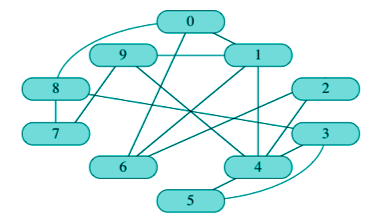
\includegraphics[width=0.5\textwidth]{figuras/grafo-rede-social.png}
	 \vspace{-0.2cm}
	\\\textbf{\footnotesize Fonte: Khan Academy}
	\label{fig:figura1}
\end{figure}

\subsubsection{\esp Matriz de Adjacência}

A matriz de adjacência é uma matriz quadrada usada para representar um grafo finito de  N x N onde N é o número de vértices do grafo que inicialmente é preenchida com 0, mas quando houver uma relação entre o vértice I com o vértice J, essa ligação é marcada com 1. Assim sendo, dado um grafo G com N vértices, pode-se representá-lo em uma matriz A(G)=[aij].
A definição precisa das entradas da matriz varia de acordo com as propriedades do grafo que se deseja representar, porém de forma geral o valor Aij guarda informações sobre como os vértices Vi e Vj estão relacionados. 

Elementos diagonais da matriz são nulos, uma vez que as arestas de um vértice que apontam para si mesmo não são permitidas em grafos simples. O mesmo conceito pode ser aplicado para multigrafos e grafos com loops em que se é armazenado o número de arestas entre cada dois vértices no elemento da matriz correspondente e permitindo elementos diagonais diferentes de zero. Os loops podem ser contados uma vez (como uma única aresta) ou duas vezes (como duas incidências de vértice-aresta), desde que uma convenção consistente seja seguida. Os grafos não direcionados geralmente usam a última convenção de contar loops duas vezes, enquanto os grafos direcionados geralmente usam a primeira convenção.

A transformação do grafo apresentado na figura 7 em sua representação de matriz ficaria da seguinte maneira:

\begin{figure}[ht]
	\centering	
	\caption[\hspace{0.1cm}Matriz de adjacência de uma rede social.]{Matriz de adjacência de uma rede social}
	\vspace{-0.4cm}
	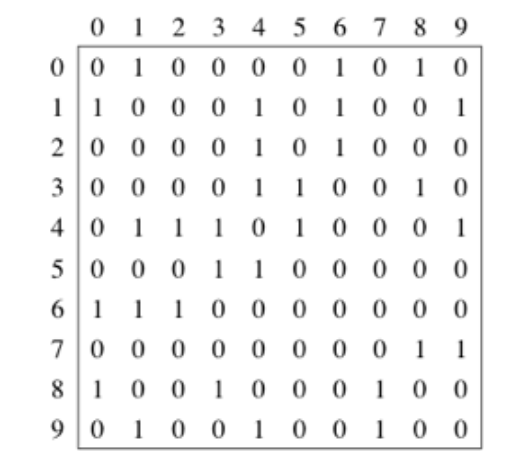
\includegraphics[width=0.5\textwidth]{figuras/matriz-adjacencia.png}
	 \vspace{-0.2cm}
	\\\textbf{\footnotesize Fonte: Khan Academy}
	\label{fig:figura1}
\end{figure}

\subsubsection{\esp Lista de Adjacência}

A lista de adjacência é algo bem comum na programação, onde se tem uma coleção de listas não ordenadas usadas para representar um grafo finito. Cada lista não ordenada dentro de uma lista de adjacência descreve o conjunto de vizinhos de um determinado vértice no grafo. Geralmente é representada com uma matriz, porque cada vértice vai precisar de um vetor diferente. Tendo em vista que não é possível ser duas vezes “amigo” de ninguém.

Uma implementação sugerida por Guido van Rossum usa uma tabela hash para associar cada vértice em um grafo com uma matriz de vértices adjacentes. Nesta representação, um vértice pode ser representado por qualquer objeto hashable. Não há representação explícita de arestas como objetos.

\begin{figure}[ht]
	\centering	
	\caption[\hspace{0.1cm}Lista de adjacência de uma rede social.]{Lista de adjacência de uma rede social}
	\vspace{-0.4cm}
	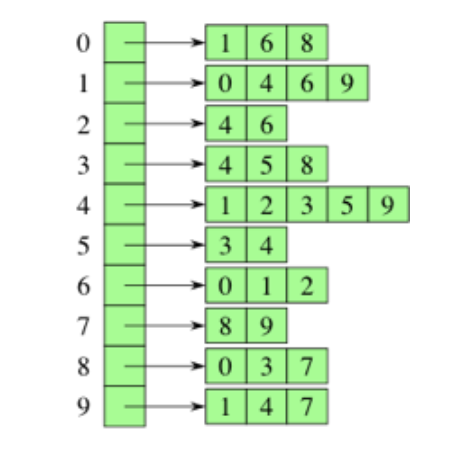
\includegraphics[width=0.4\textwidth]{figuras/lista-adjacencia.png}
	 \vspace{-0.2cm}
	\\\textbf{\footnotesize Fonte: Khan Academy}
	\label{fig:figura1}
\end{figure}

\section{\esp Algoritmos}

Um algoritmo é uma sequência de raciocínios, instruções ou operações para alcançar um objetivo, sendo necessário que os passos sejam finitos e operados sistematicamente. Um algoritmo, portanto, conta com a entrada (input) e saída (output) de informações mediadas pelas instruções.

\subsection{\esp Percurso em Grafos}

Um algoritmo de busca é qualquer algoritmo que visita todos os vértices de um grafo andando pelos arcos de um vértice a outro. Há muitas maneiras de fazer uma tal busca. Cada algoritmo de busca é caracterizado pela ordem em que visita os vértices.

\subsubsection{\esp Percurso em Profundidade (DFS - Depth First Search)}

Esta busca tem como intenção auxiliar na compreensão do grafo com que se está lidando, revelando sua forma e reunindo informações (representadas pela numeração dos vértices) que ajudam a responder perguntas sobre um determinado grafo.

Como característica principal este algoritmo visita todos vértices de um grafo, utilizando como critério os vizinhos mais recentemente visitados, utilizando de uma pilha explícita ou recursividade para guiar a busca.

Entretanto, o percurso em profundidade não resolve um problema específico. Apenas  serve como um arcabouço, ou pré-processamento, para a resolução eficiente de vários problemas concretos. Abaixo segue um exemplo de seu algoritmo:

\begin{figure}[ht]
	\centering	
	\caption[\hspace{0.1cm}Algoritmo DFS.]{Algoritmo DFS}
	\vspace{-0.4cm}
	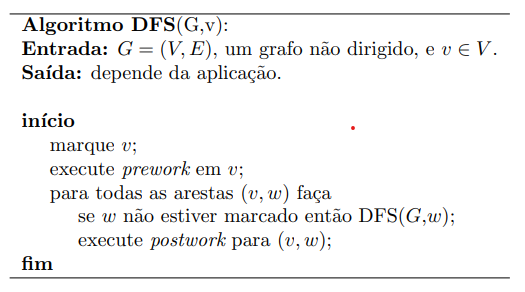
\includegraphics[width=0.7\textwidth]{figuras/dfs.png}
	 \vspace{-0.2cm}
	\\\textbf{\footnotesize Fonte:  Bondy, J. (1976)}
	\label{fig:figura1}
\end{figure}

Para cada vértice do grafo, a busca percorre todos os seus vizinhos. Assim sendo, cada aresta é visitada duas vezes.
O grafo sendo representado por uma lista de adjacências, o percurso tem
complexidade \emph{O(n + m)}.

\subsubsection{\esp Percurso em Largura (BFS - Breadth First Search)}

A busca em largura é bastante simples, pois os vértices do grafo são visitados nível a nível, ou seja, todos os vértices a uma distância k do vértice inicial são visitados antes de qualquer vértice a uma distância k + 1 do inicial.

A busca em largura produz uma árvore com raíz S e que possui todos os vértices acessíveis. Conceitualmente, ao invés de gerar uma árvore apenas, poderia gerar várias árvores, no caso de haverem mais de uma origem, mas como geralmente a busca em largura é utilizada em aplicações que calculam caminho mais curto entre dois pontos, isso não é muito comum. CORMEM et al. (2002, p. 422)

Abaixo segue um exemplo de seu algoritmo:

\begin{figure}[ht]
	\centering	
	\caption[\hspace{0.1cm}Algoritmo BFS.]{Algoritmo BFS}
	\vspace{-0.4cm}
	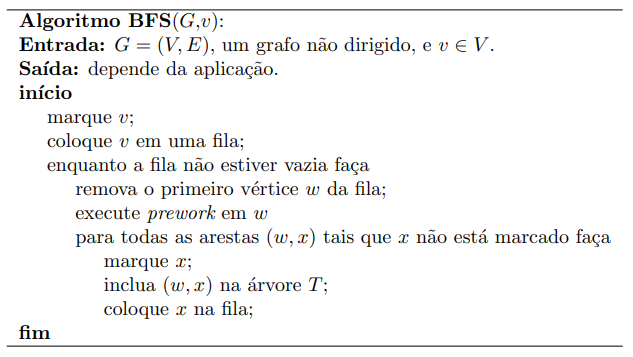
\includegraphics[width=0.7\textwidth]{figuras/bfs.png}
	 \vspace{-0.2cm}
	\\\textbf{\footnotesize Fonte:  Bondy, J. (1976)}
	\label{fig:figura1}
\end{figure}

\vspace{2cm}
\subsection{\esp Tarjan}

O algoritmo de Tarjan torna possível determinar os componentes fortemente conectados de um grafo direcionado. O algoritmo de Tarjan é linear em complexidade, como o algoritmo de Kosaraju, mas tem a vantagem de fazer apenas uma passagem no grafo em vez de duas. 
Desta forma, recebe como entrada um grafo direcionado e retorna uma partição dos vértices do gráfico correspondentes aos seus componentes fortemente conectados. 
O princípio do algoritmo é o seguinte: lançamos uma rota em profundidade a partir de um vértice arbitrário. As tuplas exploradas são colocadas sobre uma pilha P. Uma marcação específica permite distinguir certos vértices: as raízes de componentes fortemente conectados, ou seja, os primeiros vértices explorados de cada componente (essas raízes dependem da ordem em que o percurso é feito, não estão absolutamente fixadas no grafo). Quando terminamos de explorar um vértice raiz v, removemos todos os vértices até e incluindo v da pilha. O conjunto de vértices removidos forma um componente fortemente conectado do gráfico. Se ainda houver picos não alcançados no final da rota, recomeçamos a partir de um deles.

\subsection{\esp Fleury}

O algoritmo de Fleury é utilizado para a construção ou identificação de um ciclo euleriano em um grafo euleriano. Um caminho ou um circuito é dito euleriano se ele contém todas as arestas de um grafo. Um grafo que contém um circuito euleriano é um grafo euleriano. Um grafo que não contém um circuito euleriano mas contém um caminho euleriano será chamado grafo semi-euleriano.

Entretanto, a dificuldade em verificar se uma rede é Euleriana reside no grande número de sub-redes possíveis.

O grafo deve ter 0 ou 2 vértices ímpares. Um vértice ímpar é aquele em que o número de arestas que conectam o vértice a outros vértices é ímpar. Caso exista 2 vértices ímpares, teremos um caminho euleriano. Se o grafo possuir 0 vértices ímpares, tem-se um circuito euleriano. 

Se possuir 2 vértices ímpares, começa-se em um desses dois vértices. Caso tenha 0 vértices ímpares, pode-se começar em qualquer lugar.

Para encontrar o caminho, escolhe-se a borda que não é uma ponte. Uma ponte pode ser comparada a uma ponte do mundo real que conecta uma ilha ao continente. Portanto, uma ponte em um grafo é uma aresta que conecta uma parte do grafo ao resto. Então, se está em um vértice onde uma aresta é uma ponte e a outra não, escolhe-se aquela que não é uma ponte.


\section{\esp Desenvolvimento}

O projeto foi desenvolvido na linguagem de programação Python em sua versão 3.10.8 como uma biblioteca de manipulação de grafos. A biblioteca conta com as seguintes funcionalidades:

\begin{enumerate} 
\item [a)]Criação de um grafo com X vértices;
\item [b)]Criação e remoção de arestas;
\item [c)]Ponderação e rotulação de vértices e arestas;
\item [d)]Checagem de adjacência de entre vértices e entre arestas;
\item [e)]Checagem da existência de arestas;
\item [f)]Checagem da quantidade de vértices e arestas;
\item [g)]Checagem de grafo vazio e completo;
\item [h)]Busca em largura e profundidade;
\item [i)]Algoritmo de Fleury;
\item [j)]Algoritmo de Tarjan;
\item [k)] Algoritmo para leitura e escrita de arquivo.
\end{enumerate}

Estes métodos possuem as duas representações citadas nas seções anteriores (Matriz de Adjacência e Lista de Adjacência), com opção de leitura e escrita em um arquivo \emph{.csv} para armazenamento e processamento dos dados. Além desta extensão de arquivo poder ser utilizada na ferramenta software de código aberto e gratuito para visualização, análise e manipulação de redes e grafos \emph{Gephi}.

O artefato desenvolvido conta com testes unitários para verificação dos métodos implementados e sua coesão em relação a regra que deve obedecer.

A arquitetura do projeto foi desenhada da seguinte forma:

\begin{figure}[ht]
	\centering	
	\caption[\hspace{0.1cm}Arquitetura do projeto.]{Arquitetura do projeto}
	\vspace{-0.4cm}
	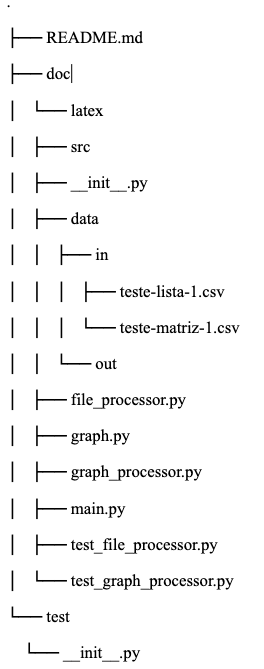
\includegraphics[width=0.4\textwidth]{figuras/organizacao-projeto.png}
	 \vspace{-0.2cm}
	\\\textbf{\footnotesize Fonte: Desenvolvido pelo autor}
	\label{fig:figura1}
\end{figure}
\vspace{2cm}

Em relação a funcionalidade da aplicação no arquivo \emph{main.py} encontra-se as inserções que devem ser realizadas via linha de comando (CLI - Command line interface) para executar as ações desejadas. Como no exemplo abaixo:


\begin{lstlisting}
    python main.py 
       --format=matriz 
       --file-in=data/in/teste-matriz-1.csv 
       --file-out=data/out/criacao-arestas-output.csv 
       --operation=criacao_arestas 
       --extra_args=2
\end{lstlisting}

Neste ponto as inserções passam pela função \texttt{main()} na qual se faz a análise (parse) dos dados de entrada com base na representação requerida através do argumento \texttt{format}. 

O argumento \texttt{operation} cuida da nomenclatura do método que será chamado na execução do sistema, onde através de uma condicional é verificado se o método existe em um mapa que também define se a função recebe ou não os parâmetros de entrada através do argumento \texttt{extra-args}.

Outros argumentos desta chamada são \texttt{file-out} e \texttt{file-in} que salvam o arquivo de entrada e saída da manipulação de um gravo.

Passado deste ponto a operação de entrada sendo localizada o arquivo \emph{graph-processor.py} gerencia parte das regras para atender a solicitação, inicializando em seu construtor o formato de entrada, o conteúdo de entrada e se possui ou não um arquivo de entrada para manipulação das informações.

\subsection{\esp Criação de um grafo com X vértices}

O trecho de código abaixo apresenta a criação de um grafo com base no argumento passado.

Criando uma lista com os vértices gerados de forma aleatória com número inteiros entre 1 e 11.000 para evitar que se tenha um vértice igual. Caso durante a geração um vértice igual ao existente seja criado, é gerado um novo número.

Para completar a execução os vértices e arestas são enviados para o arquivo \emph{graph.py} para criação de um objeto Grafo a ser manipulado.

\begin{minted}{python}
def criacao_grafo_x_vertices(self, extra_args):
    vertices = []  # Lista de vértices
    # Para cada vértice
    for i in range(0, int(extra_args)):
        # Gera um número aleatório entre 1 e 11000
        random_number = random.randint(1, 11000)
        # Se o número não estiver nos vértices
        if random_number not in vertices:
            # Adiciona o número aos vértices
            vertices.append(random_number)
        # Se o número estiver nos vértices
        else:
            # Gera um novo número aleatório entre 1 e 11000
            random_number = random.randint(1, 11000)
            # Adiciona o novo número aos vértices
            vertices.append(random_number)

    # Víncula os vertices ao primeiro vertice
    arestas = []  # Lista de arestas
    # Para cada vértice
    for i in range(1, len(vertices)):
        # Adiciona uma aresta entre os vértices
        arestas.append((vertices[0], vertices[i]))

    # Cria um grafo com as arestas e direcionado
    self.grafo = graph.Grafo(vertices, arestas, direcionado=True)  
    return self.grafo  # Retorna o grafo
\end{minted}

\section{\esp Conclusão}

Discussão dos resultados obtidos na pesquisa. É onde se colocam as observações do autor. 
Poderá também apresentar sugestões de novas linhas de estudo.

A conclusão deve estar de acordo com os objetivos do trabalho.

A conclusão não deve apresentar citações ou interpretações de outros autores.
